

\section{Defining the PL-embedding $\mathcal{H}_{1}^\diamond$}\label{sec:rect}


%Let $\mathcal{H}_1^\diamond=\mathcal{H}_1^\star$ be.
Let $\mathcal{L}_{i+1}^\star$ be a subset of the pillow $\mathcal{P}_{i+1}^\star$, formed by the part
that comes from the tail of the balloon after the i-th $bp$-move is applied, see Fig. \ref{fig:U3}.
%, see Fig. \ref{fig:001partenova}.
%In other words, $\mathcal{U}_n^\star=\{ v_0v_3^jv_1, v_0v_4^jv_3^j, v_4^jv_2v_3^j, v_2v_5^jv_3^j, v_5^jv_1v_3^j~|~ j\in \{ 1, \ldots, 2n \} \}$ 
%and $\mathcal{L}_n^\star=\mathcal{H}_n^\star \backslash \mathcal{U}_n^\star$, see Fig. \ref{fig:001partenova}.
%Note that $\mathcal{U}^\star_n$ denote the subcomplex  
%and
%$\mathcal{L}^\star_n$ denote the subcomplex formed by the tails 
%of the balloons or the part of the pillows that came from the tails of the balloons.

\begin{figure}[!htb]
\begin{center}
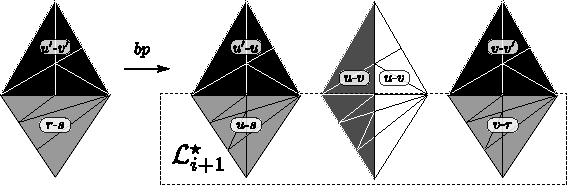
\includegraphics[width=13cm]{A.figs/U3.pdf}
\caption{The set $\mathcal{L}_{i+1}^\star$.} 
\label{fig:U3}
\end{center}
\end{figure}

%\begin{figure}[!htb]
%\begin{center}
%\includegraphics[width=14cm]{A.figs/001partenova.pdf}
%\caption{Two PL2$_3$-faces, a subset of a PL2$_0$- or PL2$_1$-face and a subset of a PL2$_2$-face (in the middle) at
% the pillow corresponding to the part that comes from the head of a balloon after all $bp$-moves be applied.}
%($\nabla_u$ and $\nabla_v$ sharing two 2-simplices in the pillow).} 
%\label{fig:001partenova}
%\end{center}
%\end{figure}


Let $\{x\} \cup Y \subseteq \mathbb{R}^N$, for $1\le N \in \mathbb{N}$. 
The \index{cone} {\em cone} \cite{rourke1982introduction} 
with vertex $x$ and base $Y$, denoted $x \ast Y \subseteq \mathbb{R}^N$,
is the union of $Y$ with all line 
segments which link $x$ to $y \in Y$.

%Let $\mathcal{U}^\star_n$ denote the subcomplex formed by the heads of 
%the balloons or the part 
%of the pillows that came from the heads of the balloons.
%Let $\mathcal{L}^\star_n$ denote the subcomplex formed by the tails 
%of the balloons or the part of the pillows that came from the tails of the balloons.
%Note that $\mathcal{H}^\star_n =  \mathcal{U}^\star_n\cup\mathcal{L}^\star_n$.

%It is now possible to use the (rectilinearly embedded into $\Pi_\ell \cup \Pi_r$) 
Now we define a PL-complex $\mathcal{H}^\diamond_1$ explicitly embedded into $\mathbb{R}^3$. 
We use the (rectilinearly embedded into $\Pi_\ell \cup \Pi_r$) 
final wings and the cone contruction to get the 
$\mathcal{H}^\diamond_1$. To this end, select a distinguished representative 
of the edges of $\mathcal{W}_n^\ell$ (resp. $\mathcal{W}_n^r$) incident to $z_3^j$ in the following way: if there is just one edge, choose it, 
otherwise the representative is the edge whose other end has the smallest indexed upper case label.
Let $R$ denote the set of representatives.

For each $e \in R$ 
%let  $v \in \{a_k,A_{k'},b_\ell,B_{\ell'}\}$ 
%be the other end of $e$.
add the two 2-simplices $z_0\ast e$ and $z_2\ast e$ (resp. the two 2-simplices 
$z_1\ast e$ and $z_2\ast e$) to  $\mathcal{H}^\diamond_1$.  
To complete 
$\mathcal{H}^\diamond_1$ add the 
2-simplices $\{z_3^jz_1z_0 \ | \ j=1,\ldots,2n\}$.
In Fig. \ref{fig:U} the solid lines
  (the edges of $R$) and the dashed edges are part of $\mathcal{L}^\star_i$,
and are treated in next section.

\begin{figure}[!htb]
\begin{center}
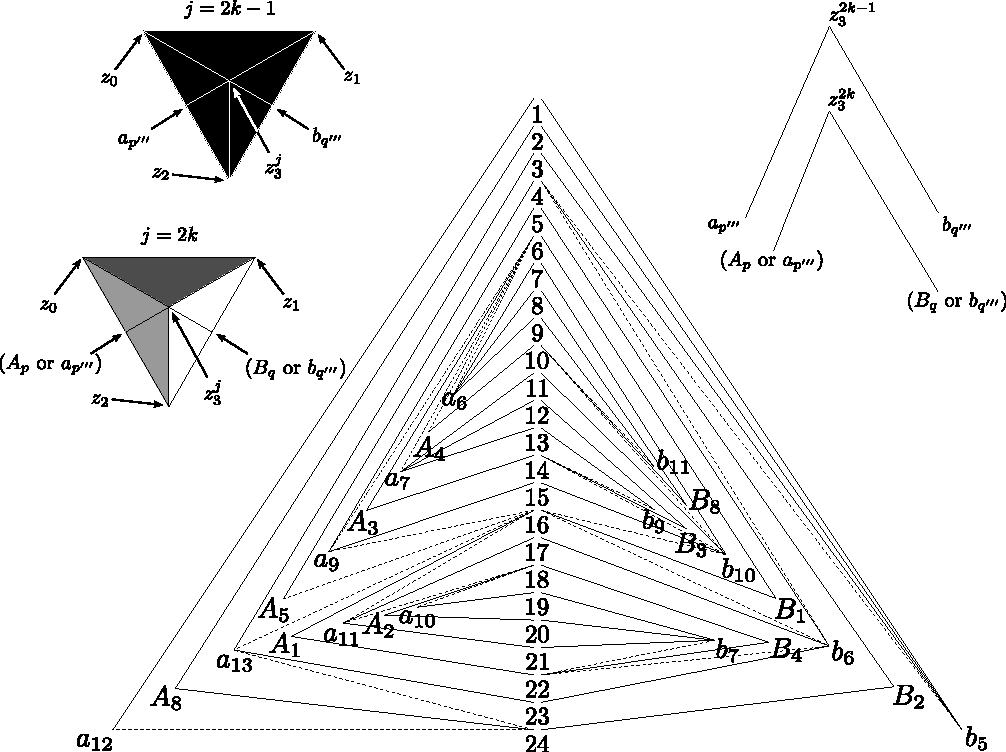
\includegraphics[width=15cm]{A.figs/U.pdf}
\caption{We use the cone construction with the solid lines to obtain $\mathcal{H}_1^\diamond.$ 
Then we use the dashed lines
to obtain the information of $z_3^\dagger$ and $a_{p'}, A_p, a_{p''}$ or $b_{q'}, B_q, b_{q''}$ 
latter when obtaining $\mathcal{L}_i^\star$. Also, we have $p'''\in\{p' ,p''\}$ and  $q'''\in\{q' ,q''\}$.} 
\label{fig:U}
\end{center}
\end{figure}

\begin{proposition}
\label{cor:embedcone}
If $\mathcal{W}_m^h$ is embedded rectilinearly in $\Pi_h$, $h \in \{\ell,r\}$,
then the pair of embeddings can be 
extended to an embedding of $\mathcal{H}^\diamond_1$ into $\mathbb{R}^3$,
via the cone construction.
\end{proposition}
\begin{proof}
 Straighforward from the simple geometry of the situation.
\end{proof}
%--------------------
%\begin{figure}
%\begin{center}
%\includegraphics[scale=1.2]{A.figs/grau.pdf}
%\caption{}
%\label{fig:grau}
%\end{center}
%\end{figure}
%--------------------






